\newpage
\section{2023秋}
\setcounter{yearcounter}{2023}

\subsection{構造工学}
\spprob{
  下に示すような、高さ$h$、幅$b$の長方形断面で、Young率$E$、Poisson比$\nu$
  の等方線形弾性材料からなる長さ$l$の棒材に、
  $x$\dspace 軸の正の方向に強制変位$g$、$y$\dspace 軸の負の方向(鉛直下向き)
  に荷重$P$が作用している。
  以下の問いに答えなさい。
  なお、荷重$P$による$x$\dspace 軸周りのねじりや強制変位$g$による
  $y$\dspace 軸及び$z$\dspace 軸回りの曲げモーメントは生じないものとする。
  また、長方形断面の断面二次モーメントは$bh^3/12$である。
  
  \begin{figure}[H]\centering
    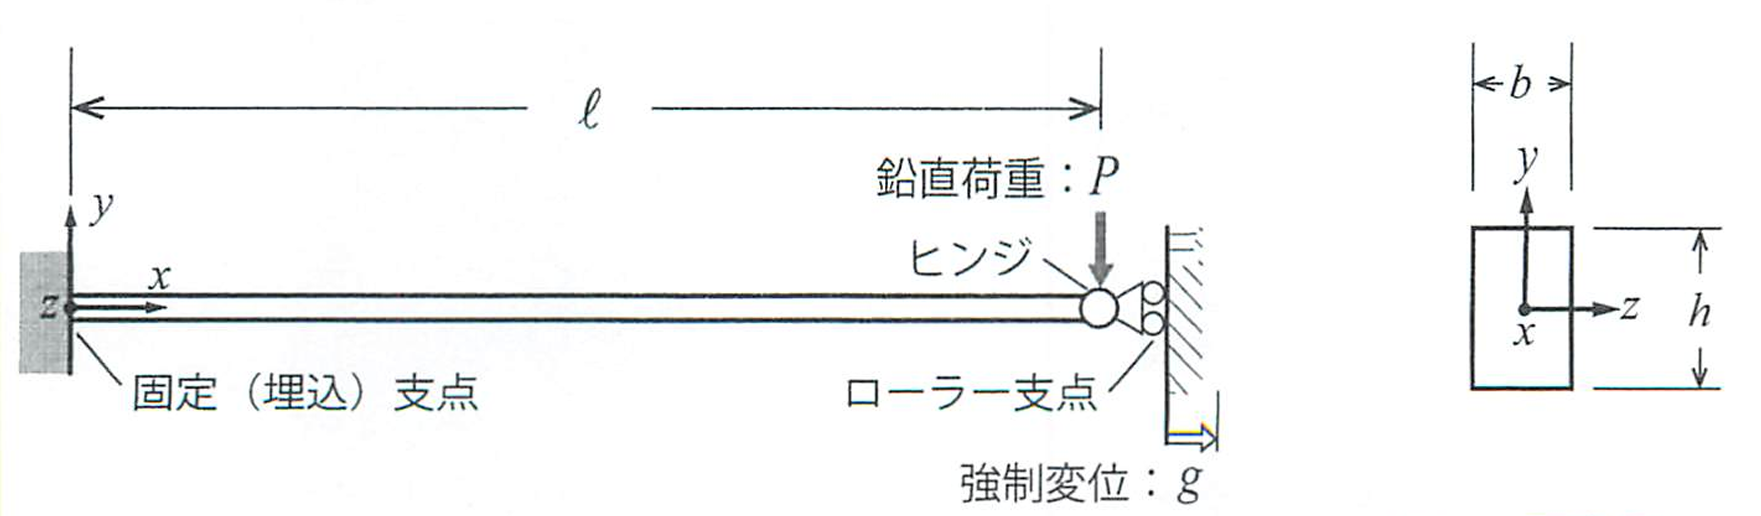
\includegraphics[width=.85\linewidth]{./src/fig/Specialized/S_2023_autumn_1.png}
  \end{figure}
  
  \begin{enumerate}[label=(\arabic*)]
    \item 強制変位$g$のみによる$x$\dspace 軸方向垂直応力を求めよ。
    ただし、$\grs_x = E\ve_x$を用いてよい。
    ここで、$\grs_x$と$\ve_x$は、それぞれ$x$\dspace 軸方向垂直応力と垂直ひずみである。
    \item 荷重$P$のみによる$x$\dspace 軸方向垂直応力の最大値および最小値と、
    それらが生じる点の$(x,y)$座標をそれぞれ求めよ。
    \item 強制変位$g$と荷重$P$が同時に作用するときの$x$\dspace 軸方向垂直応力の最大値および最小値を求めよ。
    ただし、荷重$P$の作用による曲げモーメントに強制変位$g$による長さと断面の変化の影響は考えない。
    \item $g = \SI{0.1}{mm},\, h = \SI{100}{mm},\,b = \SI{50}{mm},\,l=\SI{1000}{mm},\,P=\SI{10}{kN},\,E=\SI{200}{G Pa},\,\nu=0.0$
    のとき、問(3)で求めた最大応力および最小応力の値をそれぞれ数値で答えなさい。
    \item 問(4)の最大応力が生じた点の$xy$\dspace 面内の最大せん断応力を\si{M Pa}で答えよ。
    \item 問(4)の最大応力が生じた点に、何らかの作用により$xy$\dspace 面内せん断応力$\tau_{xy}=\SI{24}{M Pa}$が生じるとき、最大および最小主応力をそれぞれ求めよ。
    \item 問(6)の最大主応力の方向を$xy$\dspace 座標を参照したベクトル、もしくは$x$\dspace 軸から反時計回りにとった最大主応力の方向角$\grt$を$\tan 2\grt$で答えなさい。
    \item 問(4)の強制変位$g$に新たな変位$\delta$を加えて引張応力が生じないようにしたい。$\delta$を求めよ。
  \end{enumerate}
}

\subsection{コンクリート工学}
\spprob{
  \begin{enumerate}[label=\arabic*.]
    \item コンクリートの劣化の一つであるアルカリシリカ反応について以下の問いにそれぞれ100字程度で答えよ。
    
    \begin{enumerate}[label=(\arabic*)]
      \item アルカリシリカ反応による劣化メカニズムを答えよ。
      \item アルカリシリカ反応を引き起こす骨材の特徴を答えよ。
      \item アルカリシリカ反応を抑制する方法を一つ答えよ。
    \end{enumerate}

    \item プレストレストコンクリート構造の力学機構について、
    曲げを受ける梁の断面の応力状態の変化を例にとって図を使って説明せよ。
    \item コンクリートの力学的性質について以下の問いに答えよ。
    
    \begin{enumerate}[label=(\arabic*)]
      \item コンクリートの一軸圧縮試験を行ったときの応力―ひずみ関係の概形を図示せよ。
      \item コンクリートの3種類の静弾性係数の定義について、応力―ひずみ関係を用いて説明し、それぞれの静弾性係数を求める式を答えよ。
      \item 「JIS A 1149:コンクリートの静弾性係数試験方法」で定められているコンクリートの静弾性係数を答えよ。
      \item コンクリートの弾性係数は静弾性係数のほかに動弾性係数がある。動弾性係数の測定方法を説明せよ。
    \end{enumerate}

  \end{enumerate}
}


\subsection{地盤工学}
\spprob{
  \begin{enumerate}[label=\arabic*.]
    \item 土のコンシステンシー限界について、図と以下の用語を用いて説明せよ。 \\
    【液状、塑性状、半固体状、固体状、含水比】
    \item 粘土の一次元圧縮特性について、図と以下の用語を用いて説明せよ。 \\
    【圧密降伏応力、$e―\log p$線、膨潤線、正規圧密土、過圧密度】
    \item 図1はクイックサンドを再現するための実験装置である。
    試料上端を規準とする上流槽上端の高さを$h$とする。
    上流槽を$h=0$から徐々に持ち上げてゆくと、試料は一斉に有効応力を失いクイックサンドを生じる。
    ただし、各瞬間において定常状態とみなせるほど上流槽をゆっくり動かすものとする。
    試料表面を原点として、下向きに$z$\dspace 軸を取る。試料の厚さを$l$、土粒子密度を$\rho_s$、間隙比を$e$、
    重力加速度の大きさを$g$とする。また、試料は一様で飽和状態にある。以下の問いに答えよ。
    \begin{enumerate}[label=(\arabic*)]
      \item 試料の密度$\rho$を求めよ。
      \item 深さ$z$における鉛直全応力$\grs$を求めよ。
      \item 深さ$z$における間隙水圧$u$を求めよ。
      \item 深さ$z$における鉛直有効応力$\grs'$を求めよ。
      \item クイックサンドが生じるときの上流槽の高さ$h_c$を求めよ。
      \item クイックサンドが生じるときの動水勾配である限界動水勾配$i_c$を求めよ。
    \end{enumerate}
    
  \end{enumerate}
  
  \begin{figure}[H]\centering
    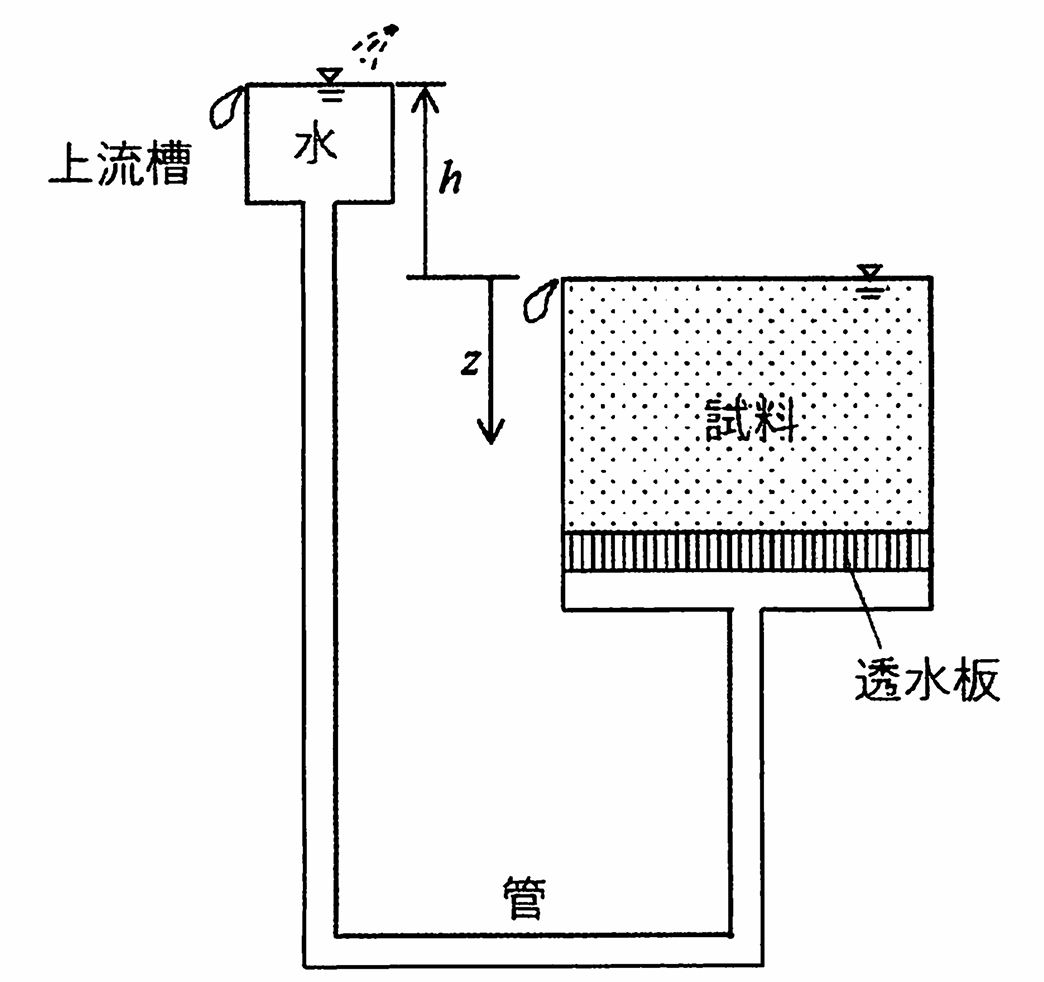
\includegraphics[width=.45\linewidth]{./src/fig/Specialized/S_2023_autumn_3.png}
  \end{figure}
  
  
}

